\section{Method}
\label{sec:approach}

This section details our approach for discovering trace links in a software repository. Our approach takes a software repository and requirements as input and extract trace links between requirements and the software issues, commits, pull requests (PRs) by analyzing the textual fields of these artifacts. Our prototype tool visualizes the trace links and other information on the repository. Figure~\ref{fig:sys-flow} presents the main steps of our approach. We publicly share the implementation of our approach in our replication package\footnote{https://zenodo.org/record/8076509}

\begin{figure}[htb]
    \centering
    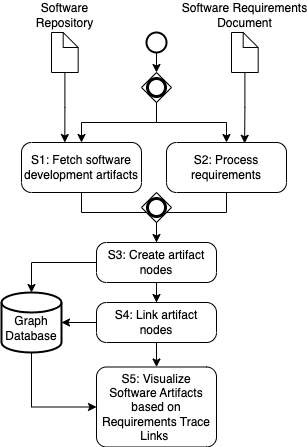
\includegraphics[width=0.65\linewidth]{figs/approach.png}
    \caption{Steps of our approach}
    \label{fig:sys-flow}
  \end{figure}

  The first two steps, \textsf{S1} and \textsf{S2}, concerns processing the two inputs of our approach, a software repository and natural language requirements, respectively. \textsf{S1} fetches issues, pull requests, and commits from a repository whose URL is given. Our prototype expects a Github repository, however our approach is general and can be applied to other repositories where the aforementioned development artifacts are present. %Table~\ref{tab:artifactfeatures} presents the attributes of these artifacts that are used in our approach.
  Our prototype expects a text file containing requirements. It do not enforce a specific for requirements and is able to process the requirements that written in a hierarchical structure, which is a common practice.

          \begin{table}
        \centering
        \caption{Attributes of software development artifacts used in our approach}
        \label{tab:artifactfeatures}
        \begin{tabular}{lllll}
          \toprule
          & Requirement & Issue & PR & Commit \\
          \midrule
          ID &\checkmark &\checkmark&\checkmark&\checkmark\\
          Title &-&\checkmark&\checkmark&-\\
          Description &\checkmark&\checkmark&\checkmark&-\\
          URL&-&\checkmark&\checkmark&\checkmark\\
          Number&\checkmark&\checkmark&\checkmark&\checkmark\\
          State&-&\checkmark&\checkmark&-\\
          Creation Date&-&\checkmark&\checkmark&-\\
          Completion Date&-&\checkmark&\checkmark&\checkmark\\
          Message&-&-&-&\checkmark\\
          Comment Count&-&\checkmark&\checkmark&-\\
          Comment List&-&\checkmark&\checkmark&-\\
          Parent&\checkmark&-&-&-\\
          OID&-&-&-&\checkmark\\
          Text&\checkmark&\checkmark&\checkmark&\checkmark\\
          \bottomrule
        \end{tabular}
      \end{table}


%The tool expects a Requirement Specification Document(RSD) in the form of a text file written in natural language, along with a URL to the GitHub repository of the software project. The software development artifacts, namely Issues, PRs and Commits are fetched from the repository leveraging the GitHub API and the requirement statements are parsed from the given RSD. This operation yields files containing information about Software Development Artifacts (SDA) and requirements, with their associated properties, such as title, description, creation and closure dates, status, and URLs. These artifacts serve as the data source for establishing trace links.

 In \textsf{S3} nodes are created for each of the requirements, issues, pull requests, and commits. 
The features  in Table~\ref{tab:artifactfeatures} are added as the node attributes. 
 Our prototype uses Neo4j\footnote{https://neo4j.com} as a graph database.

      \textsf{S4}  links the requirements to artifacts by creating edges between their associated nodes . 
      Two types of relationships are captured between the artifacts, namely \emph{tracesTo} and \emph{relatedCommit}. 
      The  \emph{tracesTo} relationship represents a trace link between a requirement node and a software development artifact node. 
      The \emph{relatedCommit} is a relation between commit and a pull request nodes. 
      This relation captures provides insight about how the commits are organized by the team. 
      In practice requirements can trace directly to commits or via pull requests (as seen in Figure˜\ref{fig:rawtracegraph}).

      We implement and evaluate three methods to extract trace links, which are represented with the \emph{tracesTo} relation. 
 The first method extracts keywords from the requirements and development artifacts and links the requirements to the artifacts that share keywords. 
 The other methods are based on the \textit{term frequency-inverse document frequency} (TF-IDF) vectors and \textit{word vectors} obtained from a pre-trained model.
For these methods, requirements are linked to the artifacts with similar vectors. 
      The overview of the processing of software artifacts to extract the trace links is shown in Algorithm~\ref{alg:process-software-artifacts}.
            \makeatletter
\algnewcommand\algorithmicswitch{\textbf{switch}}
\algnewcommand\algorithmiccase{\textbf{case}}
\algnewcommand\algorithmicassert{\texttt{assert}}
\algnewcommand\Assert[1]{\State \algorithmicassert(#1)}%
% New "environments"
\algdef{SE}[SWITCH]{Switch}{EndSwitch}[1]{\algorithmicswitch\ #1\ \algorithmicdo}{\algorithmicend\ \algorithmicswitch}%
\algdef{SE}[CASE]{Case}{EndCase}[1]{\algorithmiccase\ #1}{\algorithmicend\ \algorithmiccase}%
\algtext*{EndSwitch}%
\algtext*{EndCase}%
\makeatletter

\setphaserulewidth{0.4pt}

\begin{breakablealgorithm}
\caption{Trace links graph construction}
\label{alg:process-software-artifacts}
\begin{algorithmic}[1]
\State Input: $RSD$ \Comment{Requirement Specification Document}
\State Input: $GRU$ \Comment{Github Repository URL} 
\State Input: $M$ \Comment{Trace Extraction Method} 
\State Input: $\tau_{e}$ \Comment{Threshold for Vector-Based Methods} 
\State Output: $TG$ : \texttt{graph} \Comment{Trace Graph}
\phase{Fetch Software Artifacts}
% \LineComment{Request from Github graphQL API}
\State $\textit{issueList} \hspace{-0.1cm} \leftarrow$  \hspace{-0.2cm} getIssues($GRU$)\label{algl:m}
\State $\textit{prList} \hspace{-0.1cm} \leftarrow$  \hspace{-0.2cm} getPRs($GRU$)\label{algl:m}
\State $\textit{commitList} \hspace{-0.1cm} \leftarrow$  \hspace{-0.2cm} getCommits($GRU$)\label{algl:m}
% \LineComment{Parse directly from given Requirement Specification Document}
\State $\textit{reqList} \hspace{-0.1cm} \leftarrow$  \hspace{-0.2cm} getRequirements($RSD$)\label{algl:m}

\phase{Create Graph with Artifacts}

  \Switch{$s$}
    \Case{$a$}
      \Assert{0}
    \EndCase
    \Case{$b$}
      \Assert{1}
    \EndCase
  \EndSwitch

% \State neo4jConnector($issue_nodes$)\Comment{}

\State $\textit{sdaList} \hspace{-0.1cm} \leftarrow$  \hspace{-0.2cm} $issueList+prList+commitList$\label{algl:m}
% \State $\textit{TG} \hspace{-0.1cm} \leftarrow$  \hspace{-0.2cm} $issueNodes+prNodes+commitNodes+reqNodes$\label{algl:m}
\State $TG \leftarrow$  \texttt{graph} 

\For{\textbf{each} $a$ \textbf{in} sdaList} \label{algl:c}
\State $TG$.addNode(a)
\EndFor \label{algl:c}

\For{\textbf{each} $r$ \textbf{in} reqList} \label{algl:c}
\State $TG$.addNode(r)
\EndFor \label{algl:c}

\phase{Extract Trace Links}

\State preprocess($reqList$, $method$)
\State preprocess($sdaList$, $method$)
\For{\textbf{each} $r$ \textbf{in} reqList}
\For{\textbf{each} $a$ \textbf{in} sdaList}
\If{$method=$ "keyword"}
\State $keywords \leftarrow$ extract(r)
\If{$a.text$ contains any $kw$ in $keywords$}
\State $TG$.addEdge(r,a)
\EndIf
\EndIf
\If{$method=$ "vector-based"}
\State r-v $\leftarrow$ createVector($r.text$)
\State a-v $\leftarrow$ createVector($a.text$)
\If{sim(r-v, a-v)  $\geq$ $\tau_{e}$}
\State $TG$.addEdge(r,a)
\EndIf
\EndIf
\EndFor
\EndFor

\Return $TG$
\end{algorithmic}

\end{breakablealgorithm}

The \textit{getIssues, getPRs, getCommits} functions take a project repository  ($GRU$) and make API calls to the GitHub API\footnote{\url{https://docs.github.com/en/graphql}} to fetch a list of issues, PRs, and commits respectively. 
It fetches the properties shown in Table \ref{tab:artifactfeatures} for these software software artifacts. 
The \textit{$preprocess(list, method)$}  function takes  a list of software artifacts and a method for trace link creation. 
It lemmatizes the text property of each artifact in the list. 
If the method is vector-based then it also removes the stopwords. 
Thereafter, the trace links are determined according to desired method.
In the keyword based method shared keywords between the requirements and software artifacts are sought. In vector based methods the requirements and artifacts are vectorized and their similarities are compared. When similarities exceed a given threshold edges are formed.
For vector-based methods we utilize TF-IDF and word vectors.


% The $sEdge(req, sda, method)$  function determines whether a trace link exists between a given a requirement ($req$) and a software development artifact ($sda$) based on a trace link $method$. If  $method$ is `keyword extraction', the keywords are extracted from $req$ and $sda$ and an edge is created if they share keywords.
% If  $method$ is `vector-based' (tf-idf or word-embedding) vectors are created for  $req$ and $sda$  using their text property. 
% Then, the similarity between the vectors are calculated. 
% An edge is created if similarity value is above a predefined threshold.

 The following details the trace extraction methods referred to in the algorithm. %Fig.~\ref{fig:trace-methods} summarizes these three methods to extract trace links.

      % \begin{figure}[htb]
      %   \centering
      %   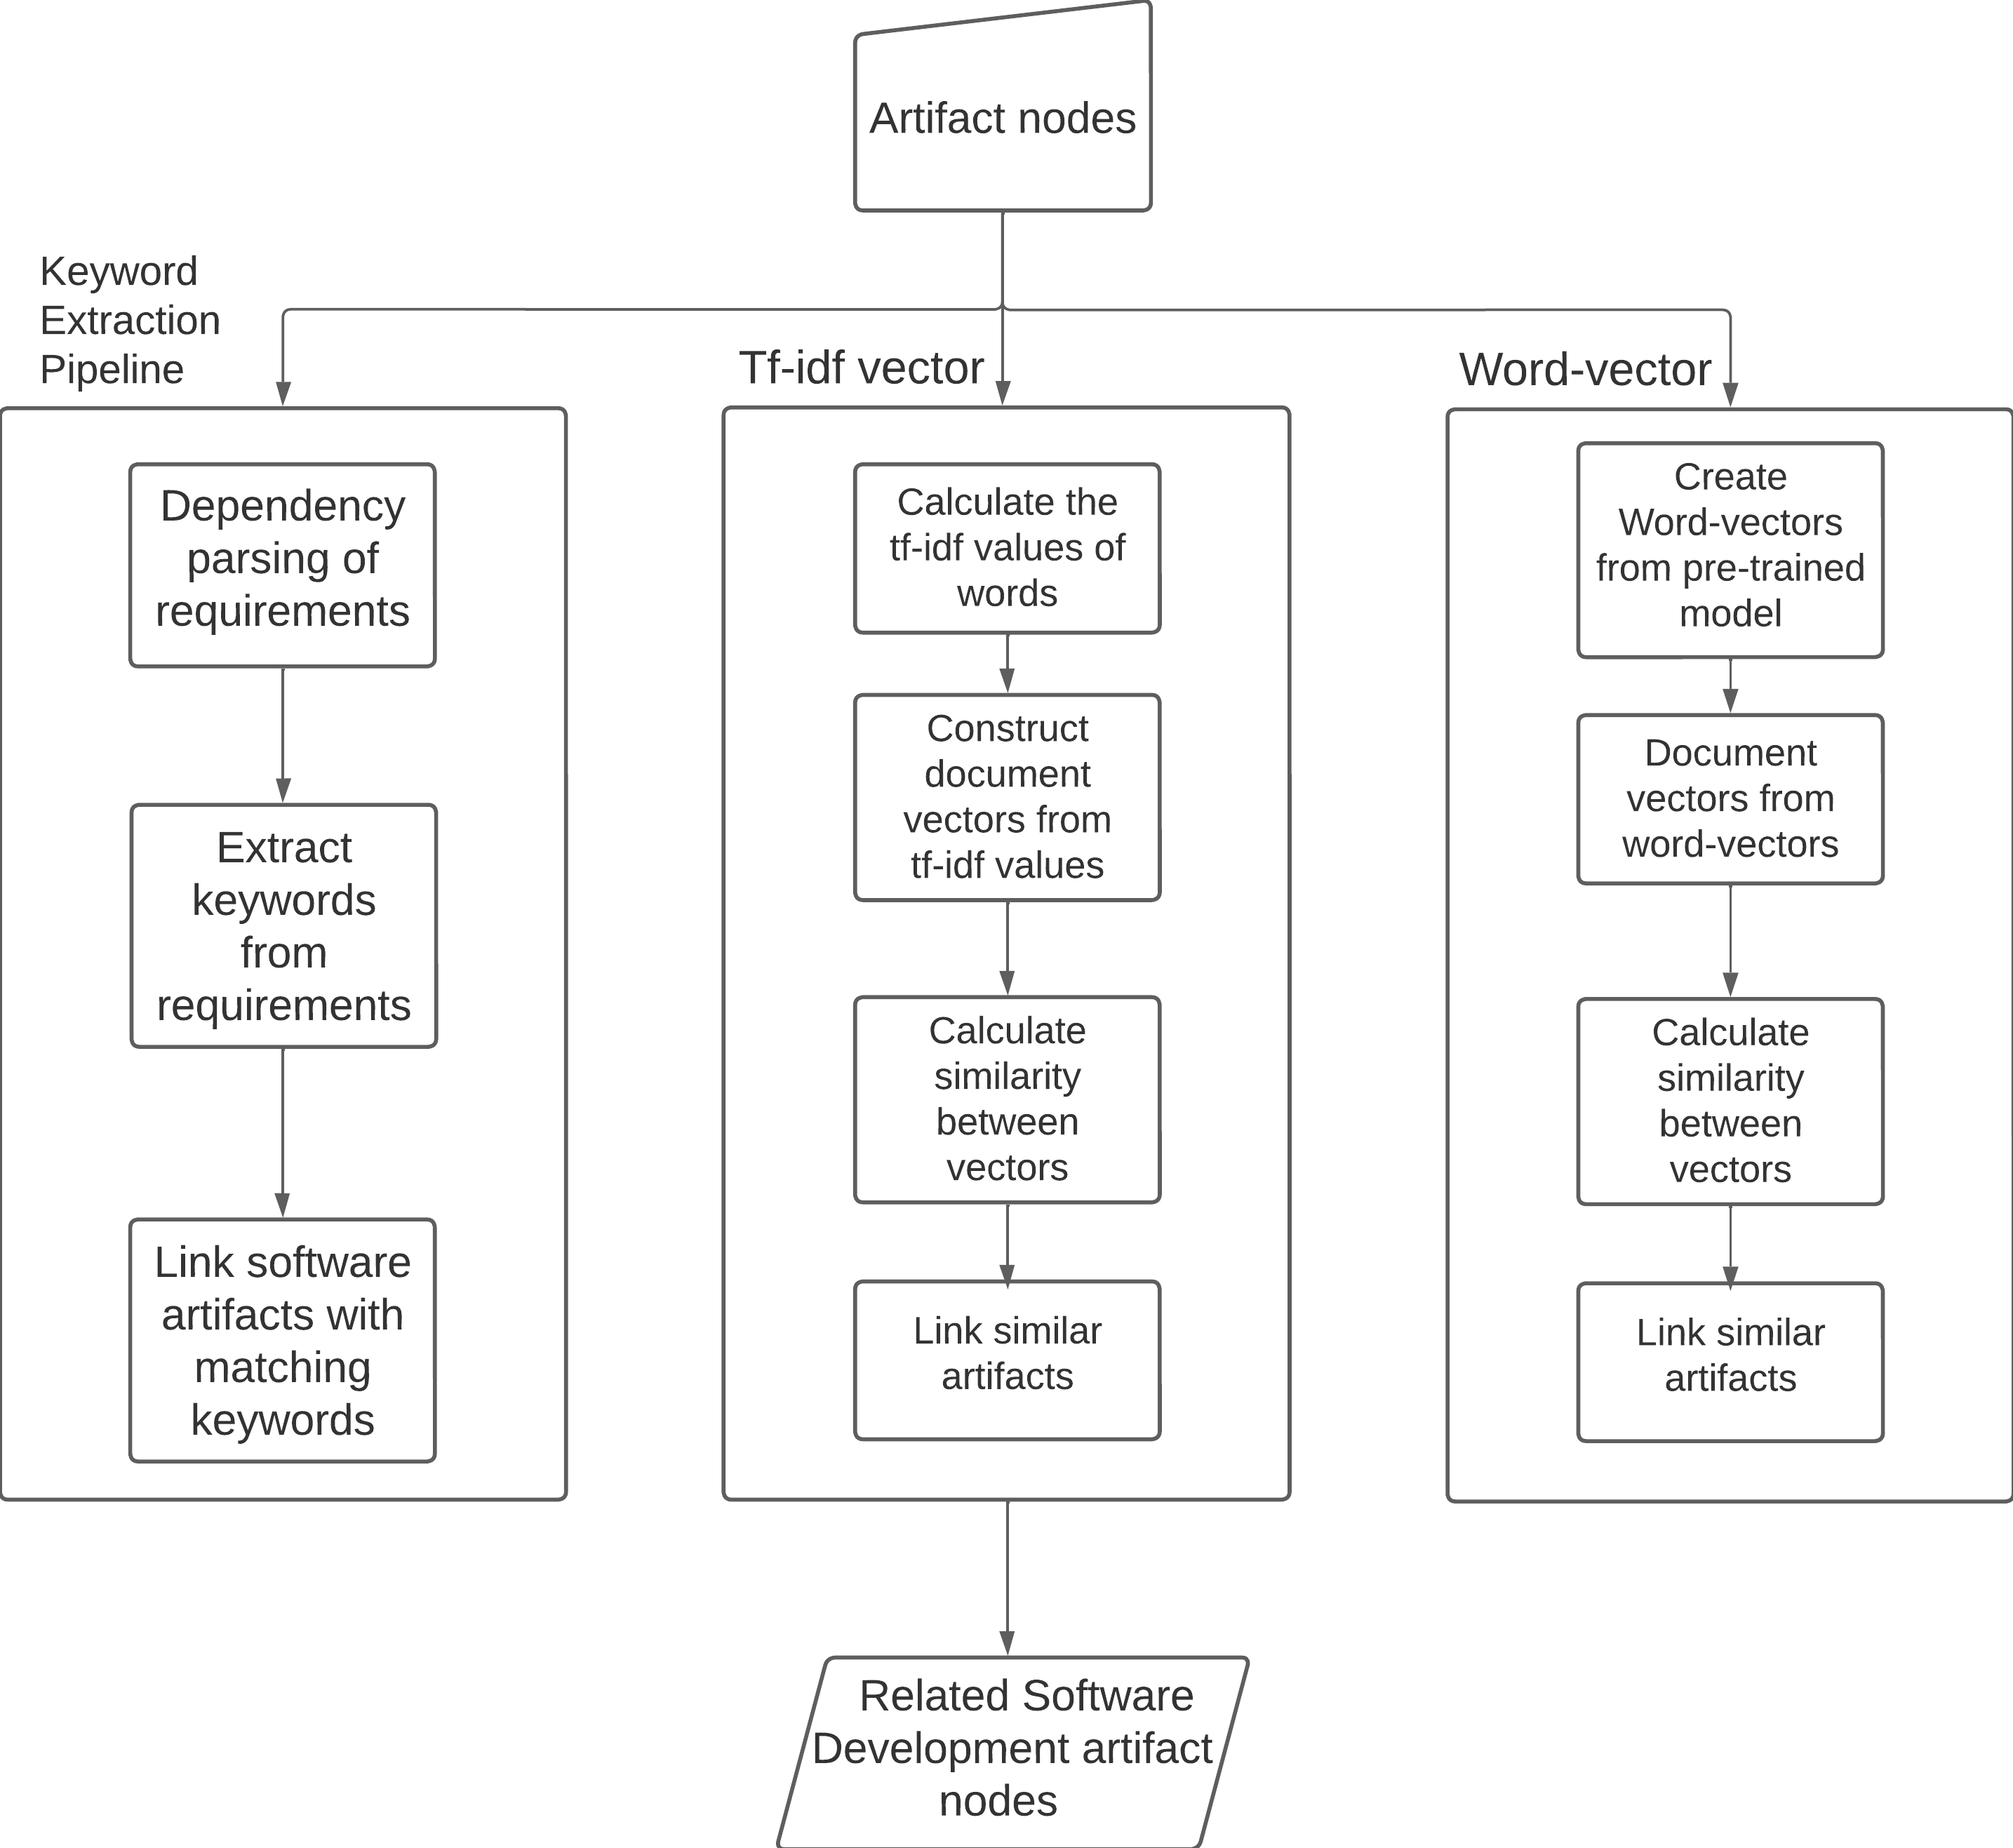
\includegraphics[width=0.9\linewidth]{figs/tracemethods.png}
      %   \caption{Control flow of the trace methods.}
      %   \label{fig:trace-methods}
      % \end{figure}

      \paragraph{Keyword Matching} To identify the most relevant keyword we combine the output of several NLP tasks that are listed below. We identify the keywords from the requirements as our trace link direction is from requirements to the software development artifacts.
      \begin{itemize}
      \item \textit{Tokenization}: We first split the natural language text of requirements.
      \item  \textit{Part-of-Speech Tagging}: We categorize each word to its correct morphosyntactic category by assigning part-of-speech (POS) tags. We focus on nouns, noun phrases, and verbs in our work to identify relevant keywords.

      \item  \textit{Dependency parsing}: We build the dependency trees of sentences to analyze the dependencies between the words of a sentence as shown in Fig.~\ref{fig:deptree}. In this tree structure, we focus on objects and create pairs of verbs and their objects called \emph{verb-objects}, and nouns and their objects called \emph{noun-objects}. We also analyze the indirect objects and conjunctions of the sentences to build these pairs.

      \item  \textit{Stopword removal}: We remove the English stopwords from the pairs we create.

      \item  \textit{Project stopwords removal}: Optionally, we allow the user to select her own stopwords for the project that may not create meaningful links such as the word event for an event management system. In such a project, the word event may create noise for it is likely to be used many requirements and development artifacts.
      \end{itemize}

      % \begin{figure}[htb]
      %   \centering
      %   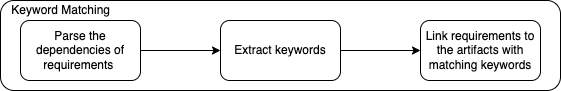
\includegraphics[width=0.99\linewidth]{figs/keywordmatching.png}
      %   \caption{Steps of trace link extraction based on keyword matching}
      %   \label{fig:keymatch}
      % \end{figure}

\begin{figure*}[htbp]
    \centering
    
\includegraphics[width=1\linewidth]{figs/displacy.png}
    \caption{The dependency tree of a requirement.}
    \label{fig:deptree}
  \end{figure*}

  Using these NLP tasks we identify the significant keywords from requirement specifications and prepare a base for identifying trace links. Fig.\ref{fig:keywords} presents the results of the method on an example requirement with the keywords extracted and their labels.

  \begin{figure}[htb]
    \centering
    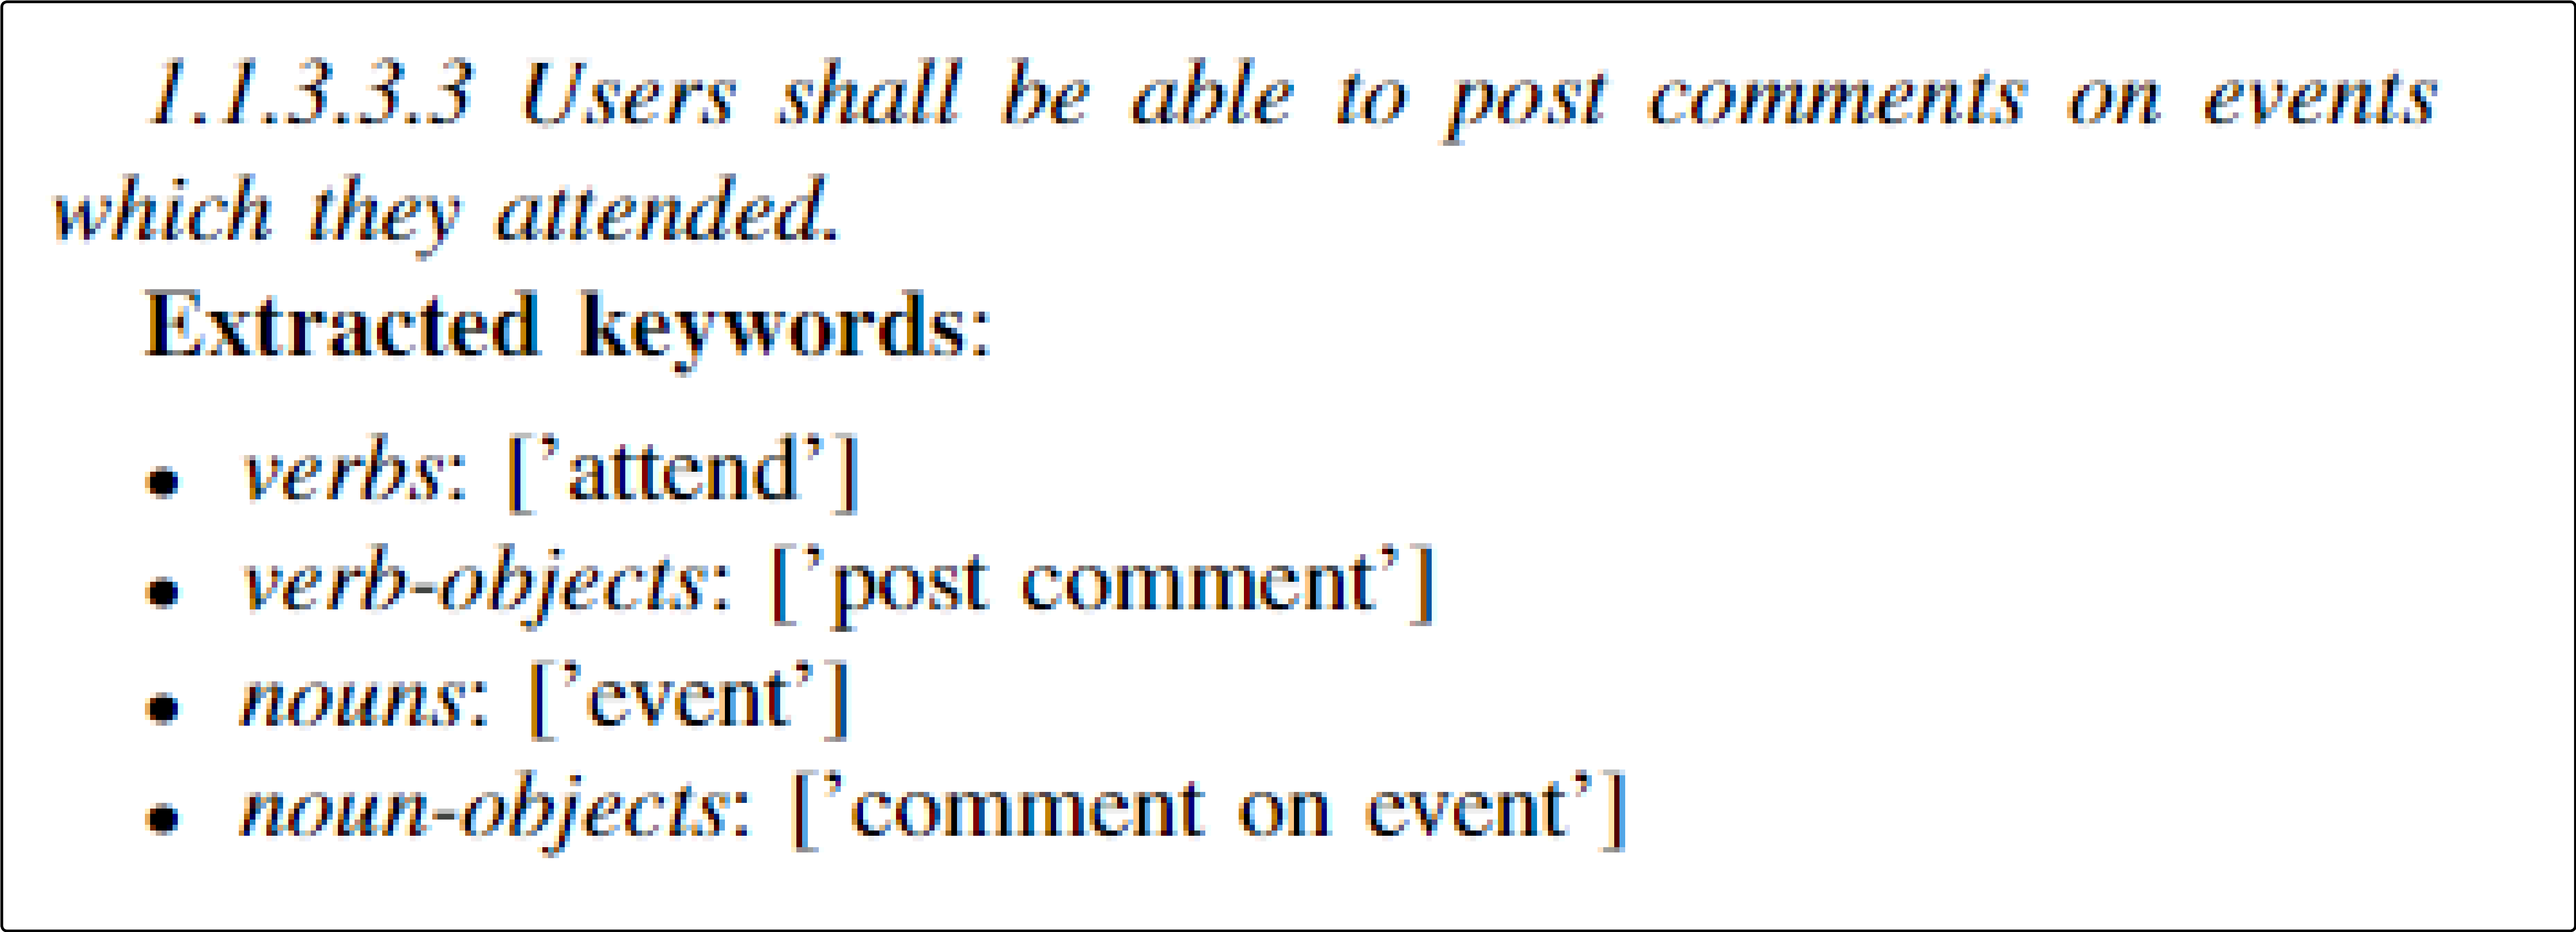
\includegraphics[width=.96\linewidth]{figs/keywords.png}
    \caption{Keyword extraction from a requirement.}
    \label{fig:keywords}
  \end{figure}

  After identifying the relevant keywords of requirements, we match them with the textual attributes of the software development artifacts in the repository. Whe create a trace link when an artifact has at least one matching keyword. We record the link in our graph database by creating an \emph{tracesTo} between the requirement node and the artifact node.

  \paragraph{TF-IDF Vectors} We first build a corpus consisting of all words in the requirements and the software development artifacts. We remove the stop words from this corpus. We calculate the TF-IDF values using Equations \ref{eq:tf}, \ref{eq:idf}, and \ref{eq:tfidf} and construct a TF-IDF vector for each requirement and artifact. We then link the requirements with artifacts that have a similarity score more than a threshold. In Sec.~\ref{sec:eval} we experiment with this threshold. Figure~\ref{fig:tfidfvec} presents the steps for this method.

  \begin{align}
    TF(t,d) &= \frac{\text{frequency of t in d}}{\text{total number of terms in d}} \label{eq:tf} \\
    IDF(t) &= log\frac{N}{1+df} \label{eq:idf}\\
    TF\text{-}IDF(t,d) &= TF(t,d)*IDF(t) \label{eq:tfidf}
  \end{align}

      \begin{figure}[htb]
        \centering
        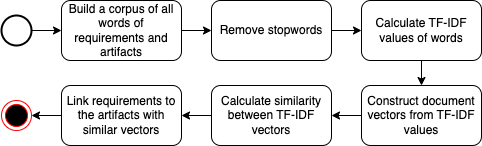
\includegraphics[width=0.99\linewidth]{figs/tfidfvector2.png}
        \caption{Steps for extracting trace links based on TF-IDF vectors}
        \label{fig:tfidfvec}
      \end{figure}

      \paragraph{Word Vectors} To generate word vectors for each artifact we use a pre-trained word embeddings model (word2vec-google-news-300). 
      We gather the word vector for each word within an artifact from the model and to build a vector for each requirement and software development artifact we average the word vectors contained in their textual attributes. 
      To extract trace links for a requirement using TF-IDF and word vectors, we calculate the cosine similarity metric of the requirement's vector with the vectors of other artifacts. 
      The artifacts that have similarities above the decided threshold are recorded as identified traces. 
      Figure~\ref{fig:wordvec} presents this method.

       \begin{figure}[htb]
        \centering
        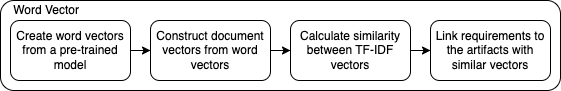
\includegraphics[width=0.99\linewidth]{figs/wordvector.png}
        \caption{Steps of trace link extraction based on word vectors}
        \label{fig:wordvec}
      \end{figure}



\begin{figure}[htb]
    \centering
    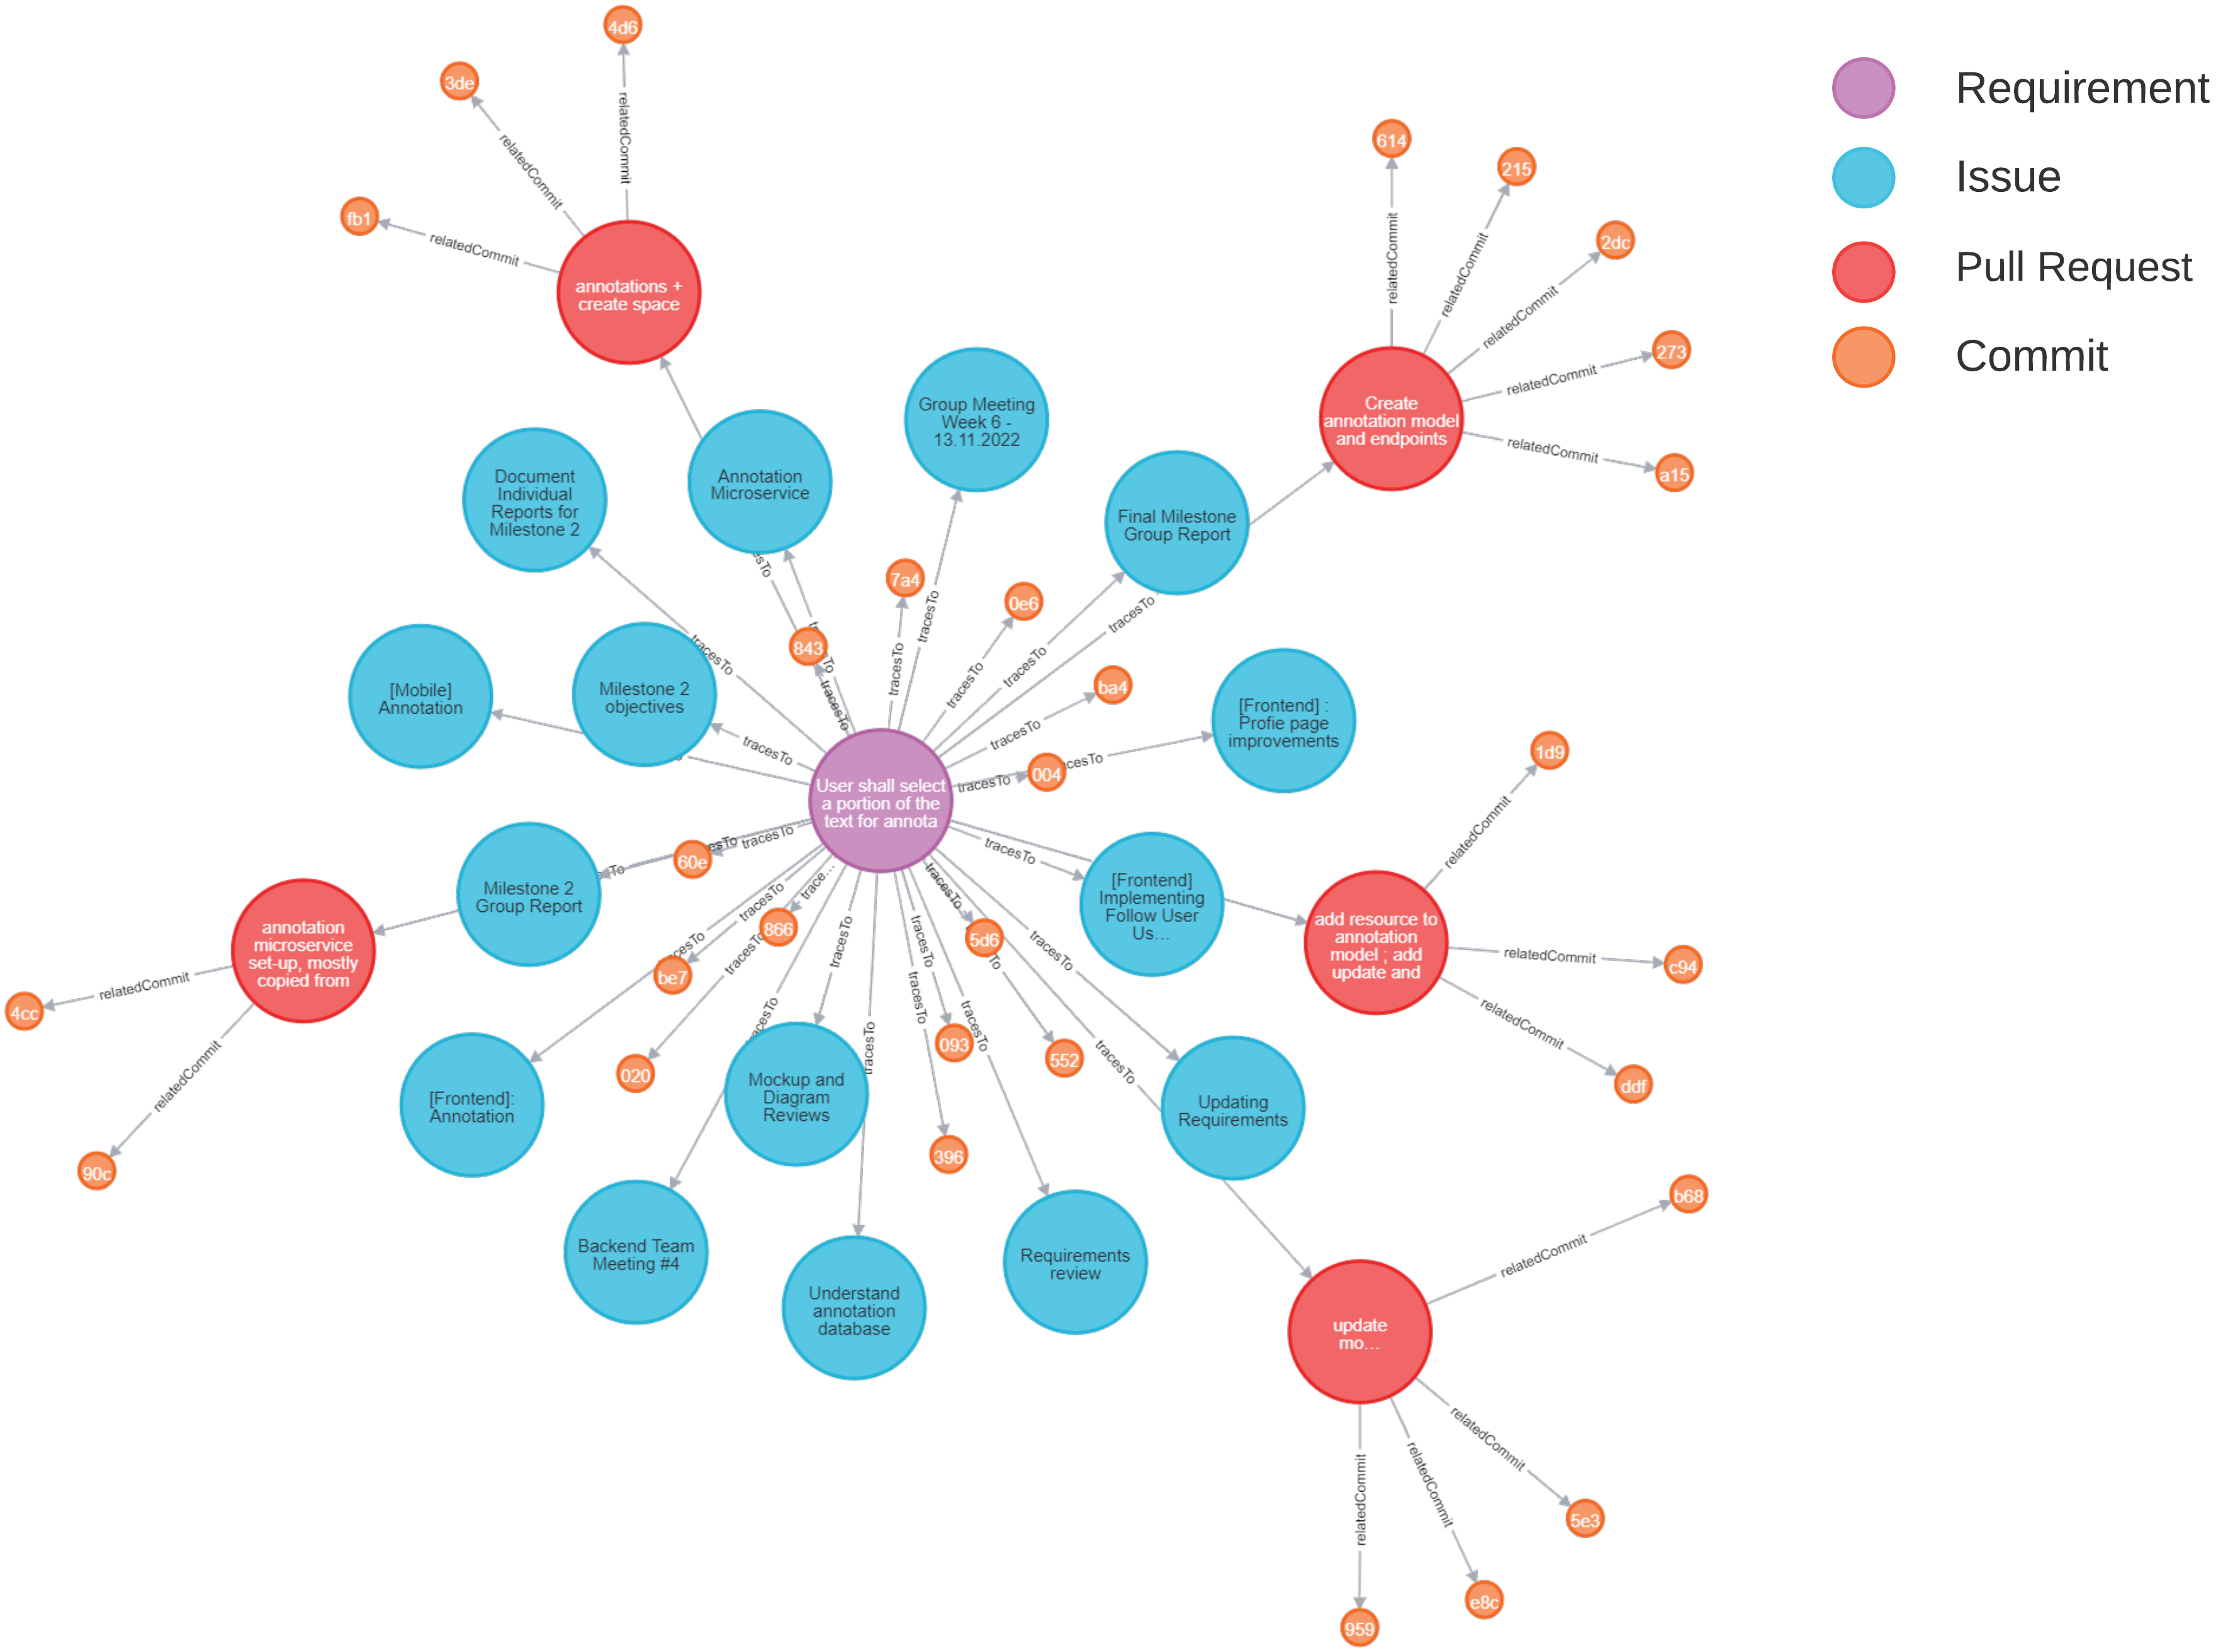
\includegraphics[width=1\linewidth]{figs/rawTraceGraph.png}
    \caption{A segment of a trace graph.}
    \label{fig:rawtracegraph}
  \end{figure}

  We add the \emph{tracesTo} relations to our trace graph based on the extracted trace links. We also add the \emph{relatedCommit} relations between the pull request (PR) nodes and the commit nodes based on the structure of the software repository we analyze. Fig. \ref{fig:rawtracegraph} illustrates a segment of the trace graph obtained from the Neo4j graph database for a specific requirement and displays the associated trace links and related commits.

\begin{figure}[htb]
    \centering
    
\includegraphics[width=.99\linewidth]{figs/traceGraph.png}
    \caption{A segment of a trace graph on a time axis.}
    \label{fig:tracegraph}
\end{figure}

The trace graph itself serves as an effective visualization of the software development artifacts (SDA) that are traced from a requirement. Moreover, it has the potential to display the lifetime of the requirement when the traced SDA are organized chronologically. In Fig. \ref{fig:tracegraph} the related SDA are arranged along a time axis based on their \textit{creationDate} property in order to represent notable information about the stages of implementation. 
For example, it is observed in the figure that the first Pull Request related to the requirement was created in week 8, while the issues concerning the planning of the requirement were created in the early stages of the development. Such visualization is useful during the development phase as well as a retrospective analysis of the software project.




% - The requirement to be examined is the root.
% - The requirement is connected to its related SDAs with \textit{tracesTo} links.
% - Pull request nodes have related commit nodes connected with \textit{relatedCommit} link.

% Who looks at trace?\\
% Trace graph can help a project manager or a developer
% Why?\\
% What can be found?


% A project manager looking at the trace graph can identify:

% \begin{itemize}
%     \item The planning phase of this requirement goes back to week 1
%     \item The implementation of this feature started at week 8
%     \item This requirement took around 13 weeks of work??
%     \item ...
% \end{itemize}

% \pagebreak

% Or in the case of a problem or a bug related to annotation, for example, a developer can view the trace of the requirement about annotation, localizing the search for the problem. Lets say the problem is about updating annotations. Looking at the trace graph, an educated guess can be made, with the information about the problem, to look at a specific pull request. For example, in our case user can view \textit{"Create annotation model"} and \textit{"... add update and delete annotation endpoints..."} nodes. Both nodes can be further observed by using the url property, reaching the github page and examining the code related to them.



Finally, \textsf{S5} provides a visualization where the user can browse the software development artifacts based on the trace links. 
We report several types pf information extracted from the repository to support software development project management. 
Neodash\footnote{\url{https://neo4j.com/labs/neodash/}} is integrated to our Neo4j graph database to provide an interactive dashboard to explore the trace graph.

The dashboard presents information about a software repository and enable the exploration based on trace links.
First, an overview of the software artifacts for a software repository.  
The number of issues and pull requests are visualized in a stacked bar chart per week to view the project progress over time. 
Similarly, the number of  issues closed per week are visualized with stacked bar chart. 
The dashboard also shows the total number of open/closed issues, open/merged PRs, and the average number of trace links per requirement. 
These statistics serve as a snapshot of the current state of the project. 
Fig.~\ref{fig:barcharts} shows the dashboard with for a repository.


%In order to reinforce the visualization of traceability data, our research includes the development of an interactive dashboard, which offers various reports that display statistical insights. Each of these reports was carefully selected to effectively visualize the corresponding data, hence they have user-friendly designs for enhanced comprehension. Moreover, many of these reports are interactive and they allow users to trace the specific requirements, thereby enabling a more customized exploration of the traceability information. The dashboard was implemented using Neodash technology, to provide full integrity with the traceability graph that is stored in the Neo4j database.

% The first report featured in Fig. \ref{fig:barcharts} is a stacked bar chart showing the number of created Issues(in green) and PRs(in brown). It could be observed that the highest number of created artifacts were in week 3 and week 7. The next report is another stacked bar chart that represents the number of artifacts opened and closed per week. Both of these charts are providing information about the status of development in the project lifetime and they help to identify periods of high or low development intensity and let users observe the assessment of the overall project dynamics.

% The dashboard also provides static data regarding the number of open/closed issues, the number of open/merged PRs, and the average number of trace links per requirement. These statistics serve as a snapshot of the current state of the project.

\begin{figure}[hbt]
    \centering
    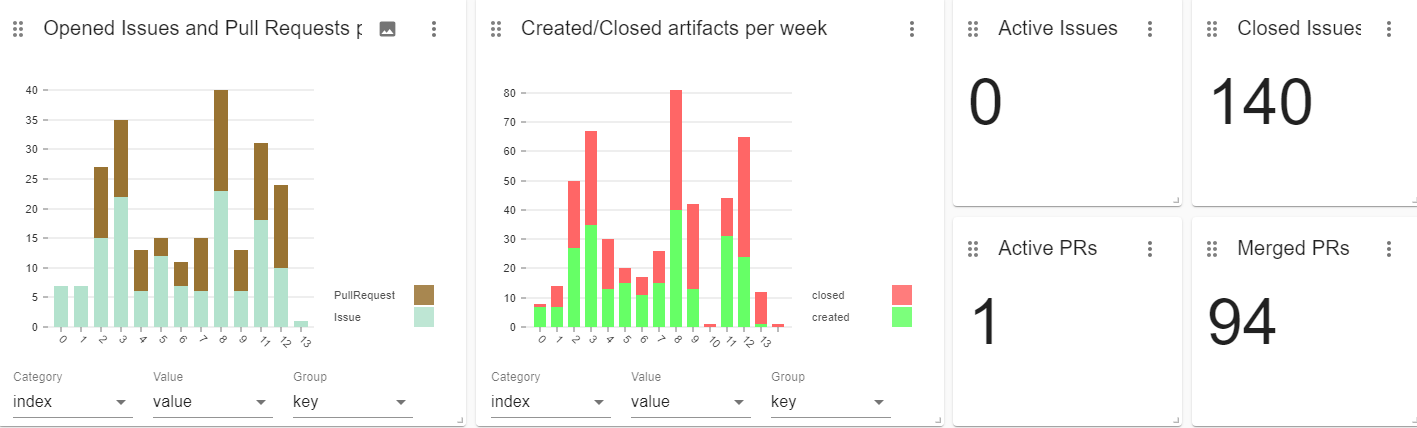
\includegraphics[width=.9\linewidth]{figs/dashboard-barcharts.png}
    \caption{Information about the software artifacts of a project. The first bar chart shows the weekly issues (red) and pull requests (brown) created. The second bar chart shows opened and closed artifacts per week.  On the right, the total number of currently active issues and PRs and completed tasks (issues and PRs). }
    \label{fig:barcharts}
\end{figure}

The dashboard displays the trace links for a requirement over the course of the project on a weekly basis to track the progress of a requirement.
It is presented using a line chart as shown in Figure~\ref{fig:linechart}. 
The project manager can visualize the data of a single requirement or compare the progress of multiple requirements. %By comparing the number of traces for each requirement, the report demonstrates the outliners, that could have relatively less or more traces.
This comparison allows the users to observe the effort associated with each requirement.%
since it displays the number of software development artifacts traced to them.

\begin{figure}[htb]
    \centering
    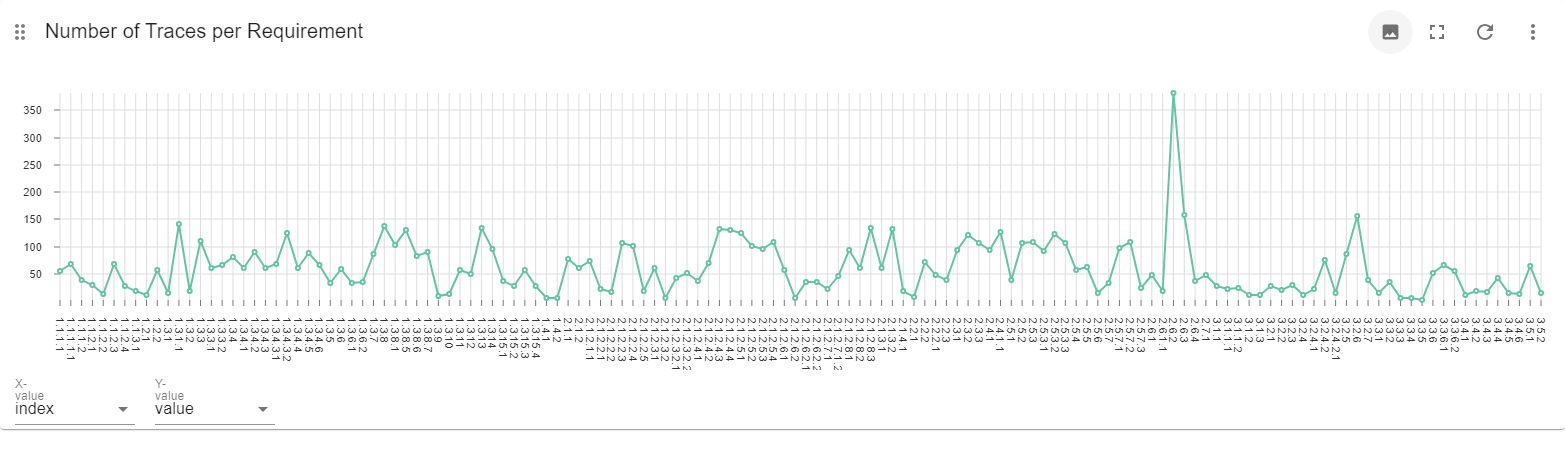
\includegraphics[width=.9\linewidth]{figs/linechart.png}
    \caption{The number of trace links for each requirement. }
    \label{fig:linechart}
\end{figure}

The dashboard shows a comparative  view of two requirements with their weighted relations to software artifacts using  a sankey diagram (Figure~\ref{fig:sankey}). % includes an example of the Sankey chart present in the dashboard that showcases the commonly traced artifacts between the chosen requirements while highlighting the strength of the trace links using the weight property.
Here, thicker lines represent a stronger relations from the requirements to their traced artifacts. 
Thus, one can see how requirements are related via their associated software artifacts.

\begin{figure}[htb]
    \centering
    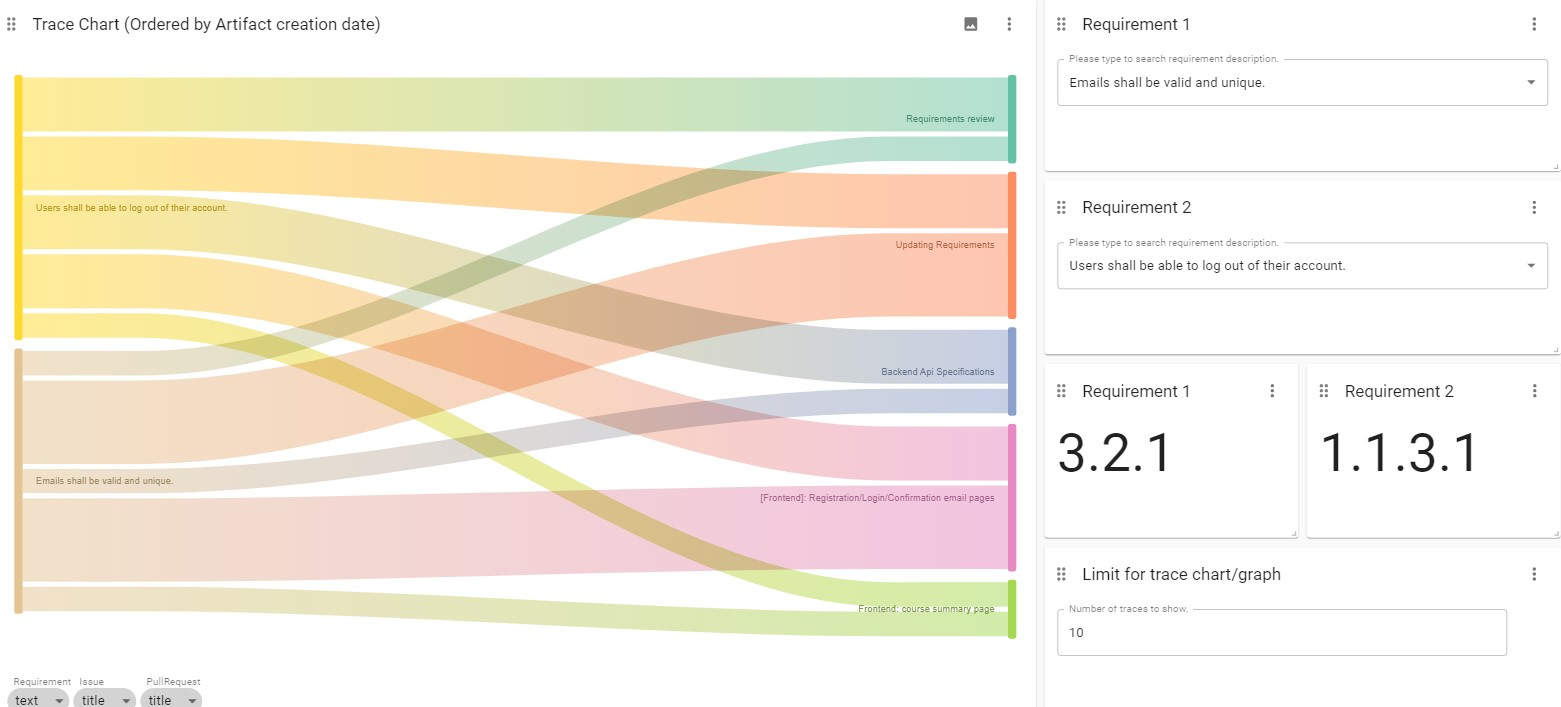
\includegraphics[width=.9\linewidth]{figs/sankey.jpg}
    \caption{The weighted relations between requirements and their associated software artifacts.}
    \label{fig:sankey}
\end{figure}

Users can interact with the dashboard to gain insights on selected requirements as seen in Figure˜\ref{fig:perreq}. 
The identified traces are presented in graphical and tabular formats for  selected requirements.
Their  current status and weekly activities are displayed in the last section of the dashboard.

\begin{figure}[htb]
    \centering
    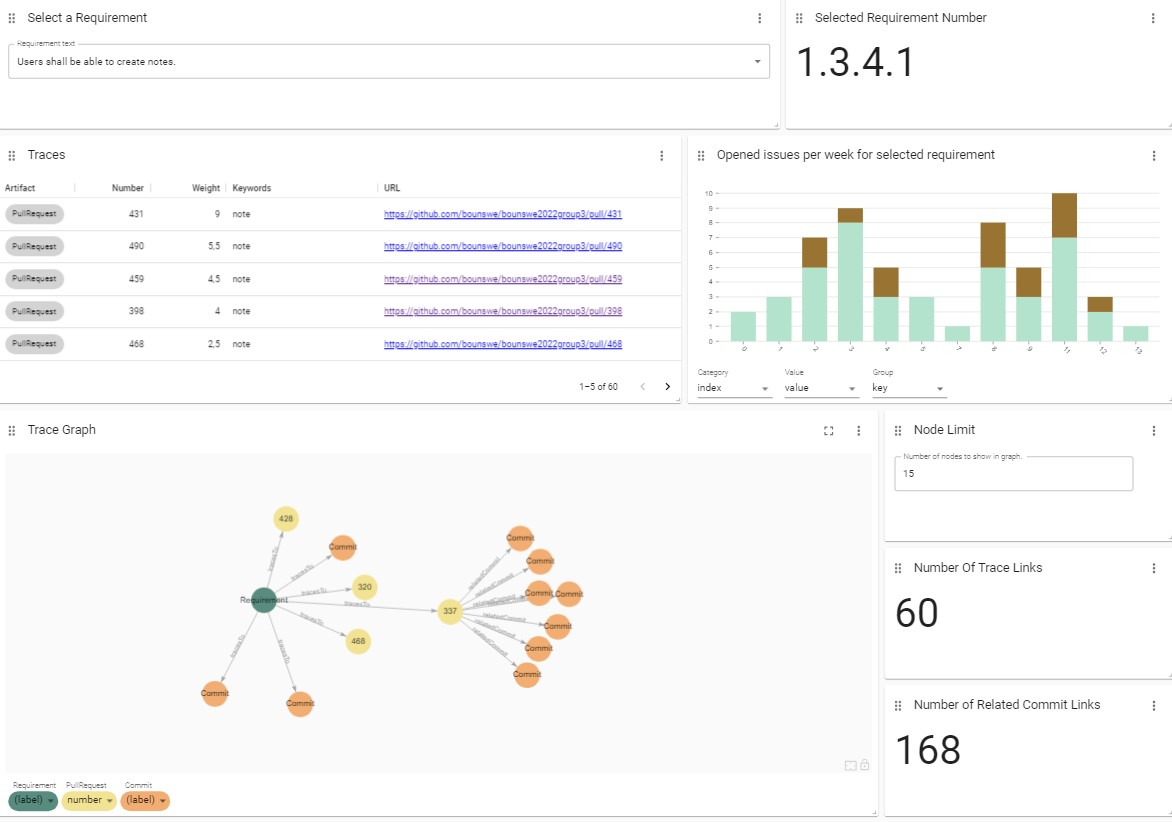
\includegraphics[width=.9\linewidth]{figs/perreq.jpg}
    \caption{Detailed information about a selected requirement.}
    \label{fig:perreq}
\end{figure}

%%% Local Variables:
%%% mode: latex
%%% TeX-master: "../main"
%%% End:
